\documentclass[10pt,mathserif]{beamer}
%\documentclass[10pt,mathserif,handout]{beamer}

\usetheme{Boadilla}
\usecolortheme{seahorse}

%\setbeamercovered{transparent}

\setbeamertemplate{section in toc}{$\circ$ \inserttocsection}
\setbeamertemplate{subsection in toc}{\hspace{1em}{\footnotesize$\circ$} \inserttocsubsection}
\setbeamertemplate{itemize item}{\scriptsize\raise1.25pt\hbox{\donotcoloroutermaths$\blacktriangleright$}}
\setbeamertemplate{itemize subitem}{\tiny\raise1.5pt\hbox{\donotcoloroutermaths$\blacktriangleright$}}
\setbeamertemplate{itemize subsubitem}{\tiny\raise1.5pt\hbox{\donotcoloroutermaths$\blacktriangleright$}}
\setbeamertemplate{enumerate item}{\insertenumlabel.}
\setbeamertemplate{enumerate subitem}{\insertenumlabel.\insertsubenumlabel}
\setbeamertemplate{enumerate subsubitem}{\insertenumlabel.\insertsubenumlabel.\insertsubsubenumlabel}
\setbeamertemplate{enumerate mini template}{\insertenumlabel}

\usepackage{fontspec}
\setmainfont[Mapping=tex-text]{Linux Libertine}
%\setsansfont{Myriad Pro}
%\setmonofont[Scale=0.9]{Consolas}
\usepackage[english]{babel}
%\usepackage[latin1]{inputenc}
%\usepackage{libertine}
%\usepackage[T1]{fontenc}

%%
\usepackage{xspace}
\usepackage{makecell}
\usepackage{msthpres}
\newcommand{\gpucb}{\textsf{GP-UCB}\xspace}
\newcommand{\gpbucb}{\textsf{GP-BUCB}\xspace}
\newcommand{\acl}{\textsf{LSE}\xspace}
\newcommand{\fullacl}{Level Set Estimation\xspace}
\newcommand{\iacl}{\textsf{LSE\textsubscript{imp}}\xspace}
\newcommand{\bacl}{\textsf{LSE\textsubscript{batch}}\xspace}
\newcommand{\ibacl}{\textsf{LSE\textsubscript{imp-batch}}\xspace}
\newcommand{\str}{\textsf{STR}\xspace}
\newcommand{\istr}{\textsf{STR\textsubscript{imp}}\xspace}
\newcommand{\bstr}{\textsf{STR\textsubscript{batch}}\xspace}
\newcommand{\rstr}{\textsf{STR\textsubscript{rank}}\xspace}
\newcommand{\var}{\textsf{VAR}\xspace}
%%

\usepackage{tikz}
\usetikzlibrary{arrows,positioning,shapes,fit}
\tikzset{
    %Define standard arrow tip
    >=stealth',
    %Define style for boxes
    st/.style={
           rectangle,
           %rounded corners,
           draw=black, thick,
           %text width=6.5em,
           minimum height=2em,
           text centered},
    % Define arrow style
    pil/.style={
           ->,
           semithick,
           shorten <=2pt,
           shorten >=2pt,}
}

\newcommand{\sig}[2]{%
\begin{tabular}{r}
#1\\[-0.7em]
{\tiny \color{darkgray}\it #2\hspace{0.5em}}
\end{tabular}}

\newcommand{\qauth}[1]{{\footnotesize\par\normalfont\hfill---\ \emph{#1}\par}}

\title[Active Learning for Level Set Estimation]
{Active Learning for Level Set Estimation}

\author[Alkis Gkotovos]{
\footnotesize
M.Sc. Thesis by Alkis Gkotovos\\
Department of Computer Science\\
ETH Zurich
}

\date[M.Sc. Thesis presentation]{
\footnotesize
Supervised by Prof. Andreas Krause

}

%\subject{Theoretical Computer Science}
% This is only inserted into the PDF information catalog. Can be left
% out. 



% If you have a file called "university-logo-filename.xxx", where xxx
% is a graphic format that can be processed by latex or pdflatex,
% resp., then you can add a logo as follows:

%\pgfdeclareimage[height=0.5cm]{university-logo}{figures/eth_logo_black.pdf}
%\logo{\pgfuseimage{university-logo}}


% If you wish to uncover everything in a step-wise fashion, uncomment
% the following command: 
%\beamerdefaultoverlayspecification{<+->}


\begin{document}

\begin{frame}
  \titlepage
\end{frame}

\begin{frame}{Outline}
  \tableofcontents
  % You might wish to add the option [pausesections]
\end{frame}


\section{Motivation and background}

\begin{frame}
\begin{center}
Swimmers of Lake Zurich, beware!\\
\vspace{0.2in}
\sig{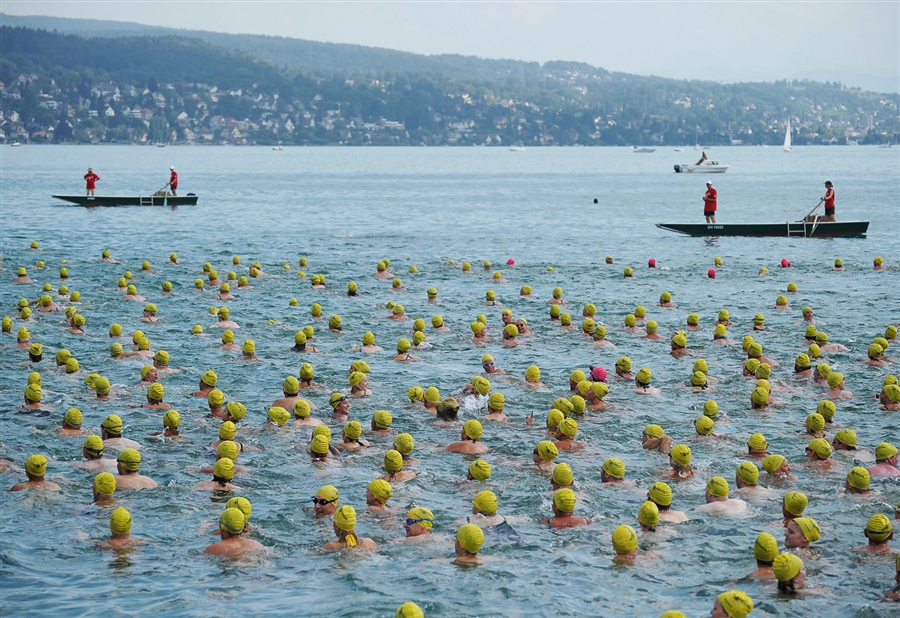
\includegraphics[width=4in]{figures/swimmers.jpg}}{Steffen Schmidt / EPA}
\end{center}
\end{frame}

\begin{frame}
\begin{center}
\uncover<1->{Swimmers of Lake Zurich, beware!}
\vspace{0.2in}
\begin{columns}[c]
\column{0.4\textwidth}
\uncover<2->{
\sig{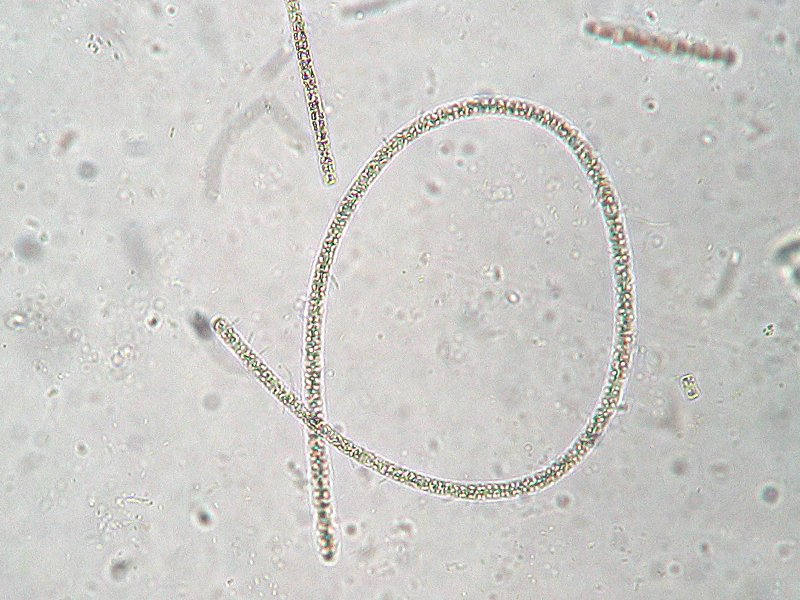
\includegraphics[width=1.7in]{figures/pr.jpeg}}{www.limnobotics.ch}\\[1em]
\sig{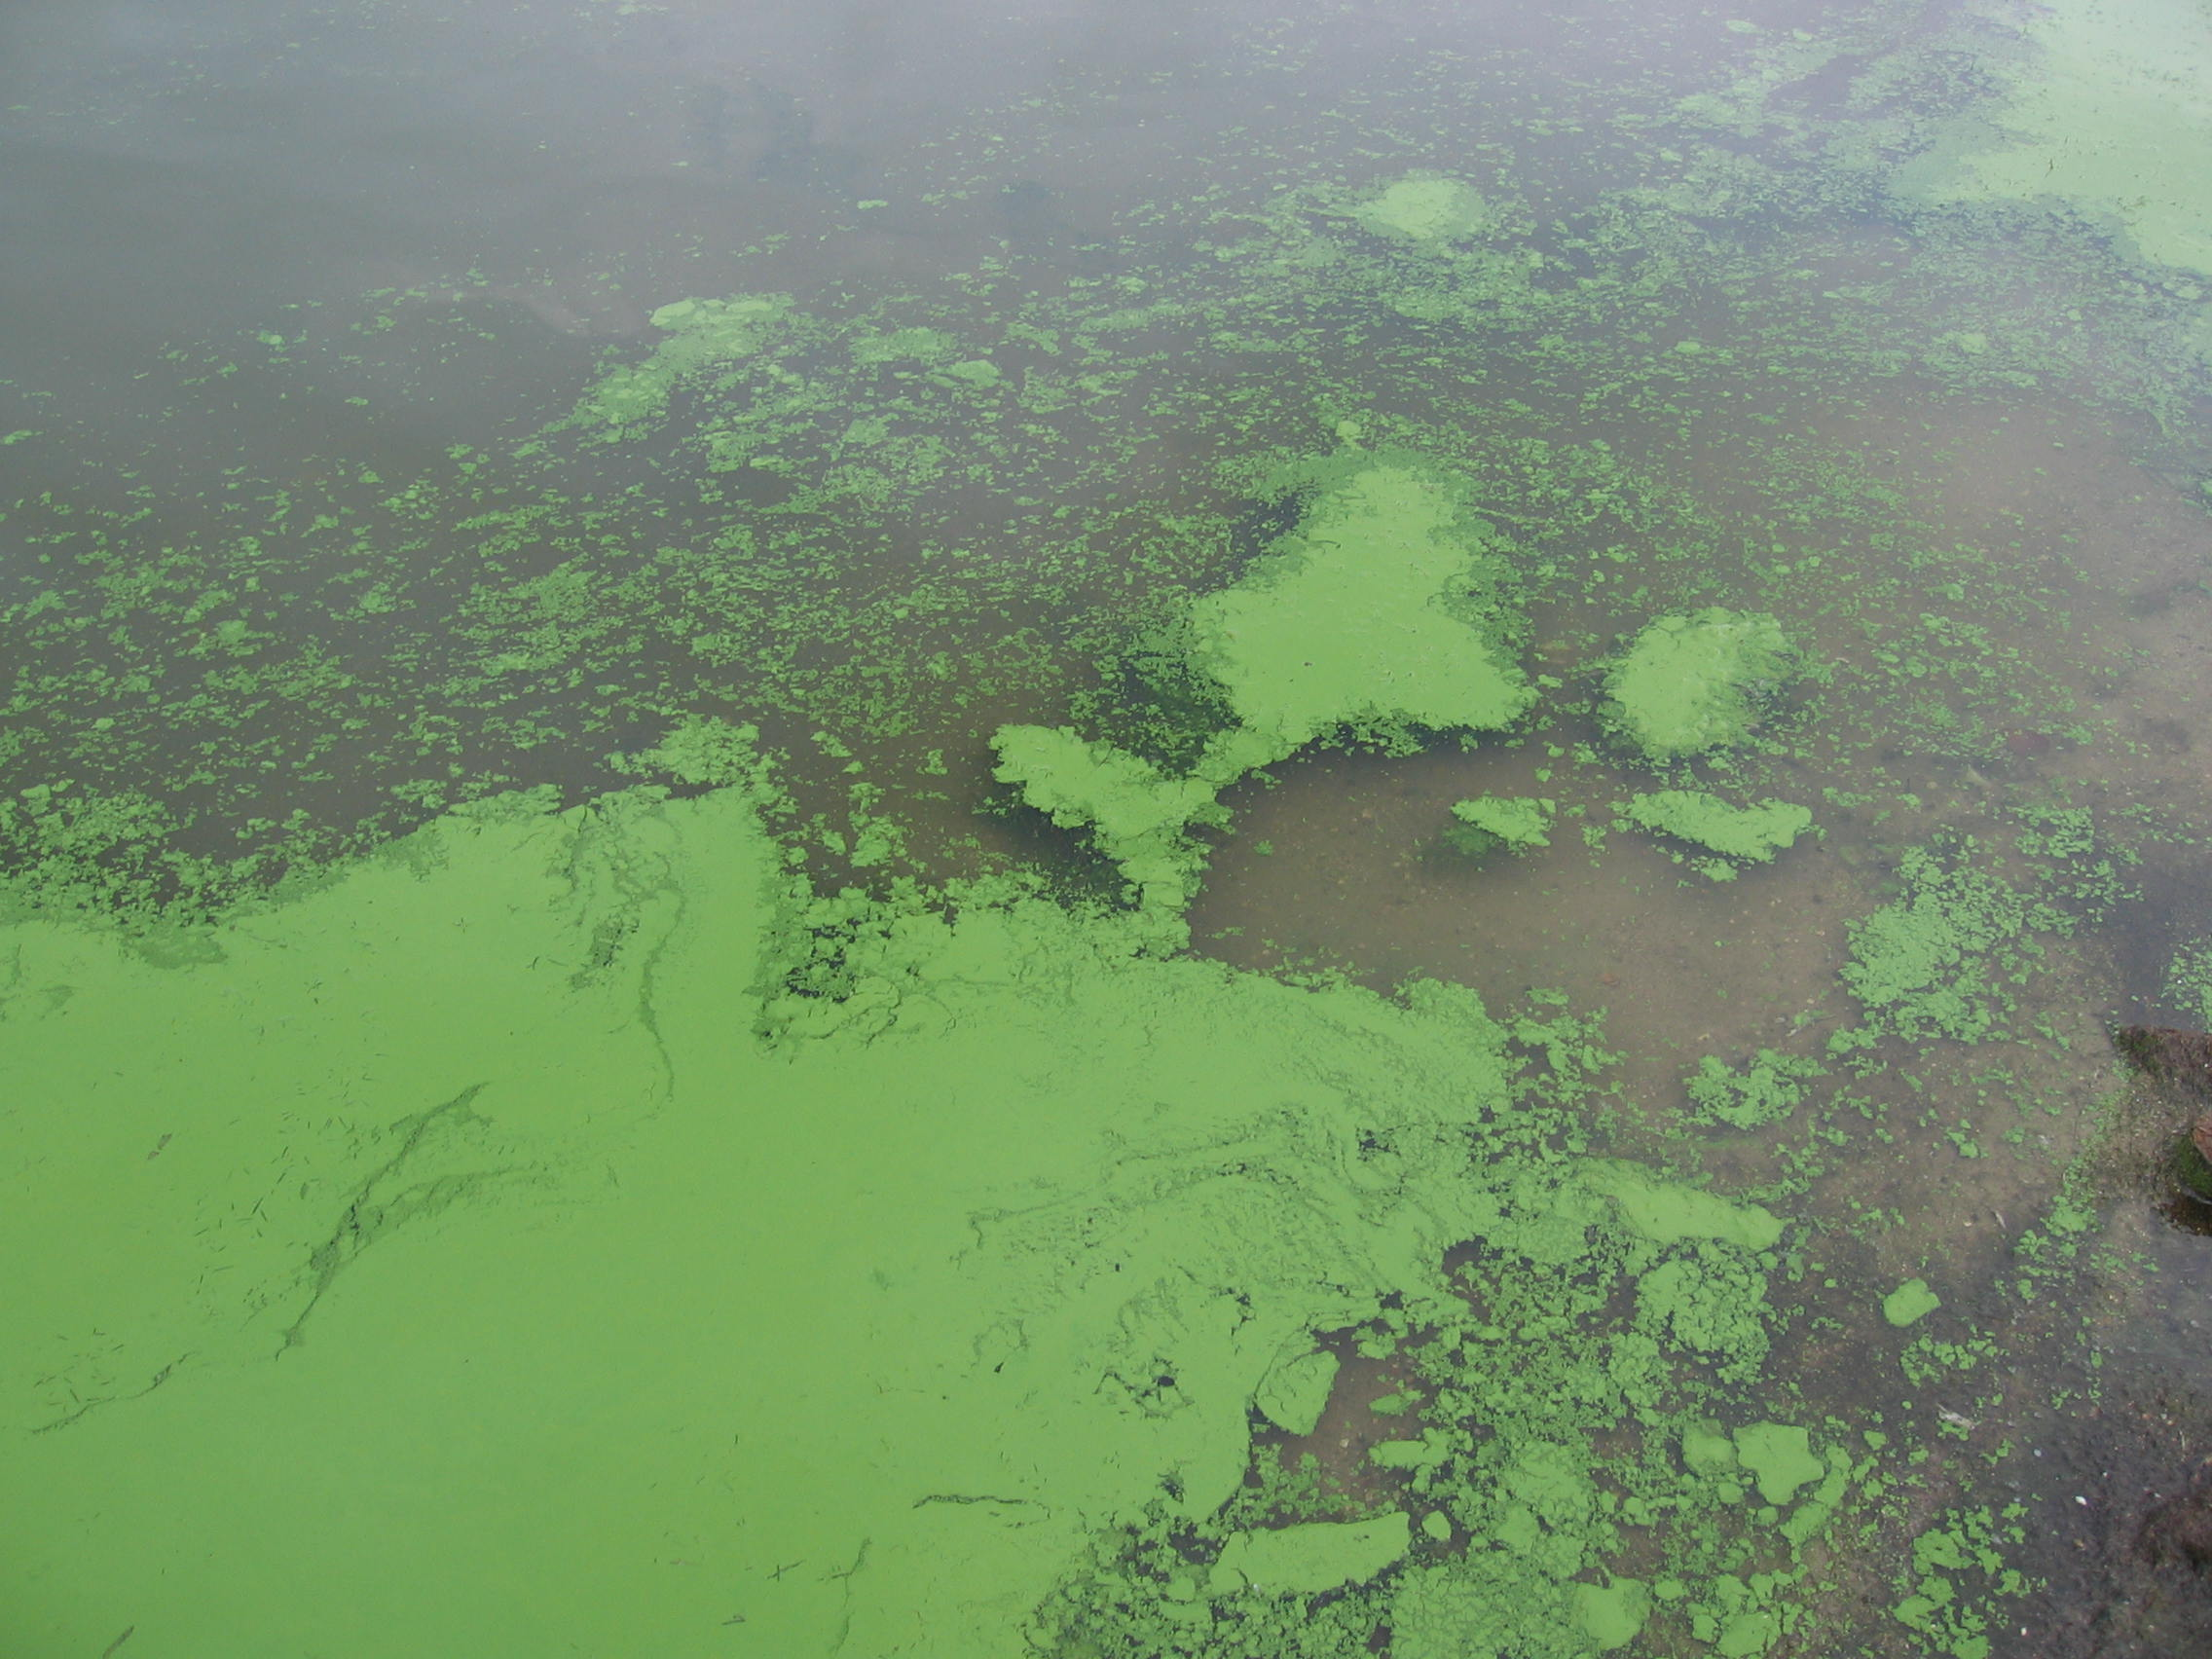
\includegraphics[width=1.7in]{figures/bloom.jpg}}{Flickr/Dr. Jennifer L. Graham/U.S. Geological Survey}
}
\column{0.6\textwidth}
\minipage[c][0.80\textheight][s]{\columnwidth}
\uncover<1->{
\small
``The warming waters of one of central Europe's most popular holiday
destinations, Switzerland's Lake Zurich, have created an ideal environment
for a population explosion of algae including \emph{Planktothrix rubescens},
[\ldots]''
\qauth{Scientific American}
}
\vfill
\uncover<3->{
\small
``\emph{Planktotrhix rubescens} can account for half of the total
phytoplankton biomass in Lake Zurich in summer [\ldots]''
\vspace{1em}

``\emph{Planktotrhix rubescens} are among the most important
producers of hepatotoxic microcystins in freshwaters [\ldots]''
\qauth{Silke Van den Wyngaert \emph{et al.}, ASLO, 2011}
}
\vfill
\uncover<4->{
\small
``Microcystins [\ldots] are cyanotoxins and can be very toxic for plants and
animals including humans.
Their hepatotoxicity may cause serious damage to the liver.''
\qauth{Wikipedia}
}
\endminipage
\end{columns}
\end{center}
\end{frame}

\begin{frame}
\begin{center}
\vspace{0.2in}
\only<1>{
\sig{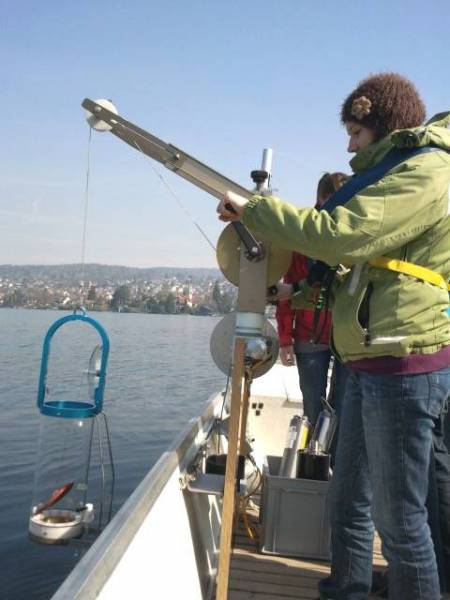
\includegraphics[width=2in]{figures/manual.jpg}}{www.limnobotics.ch}
}
\only<2>{
\sig{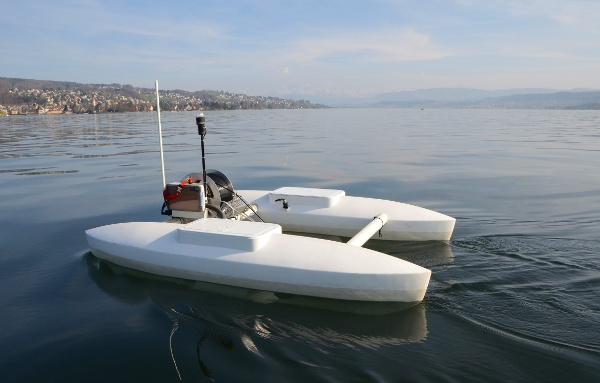
\includegraphics[width=4in]{figures/boat.jpg}}{www.limnobotics.ch}
}
\only<3>{
\sig{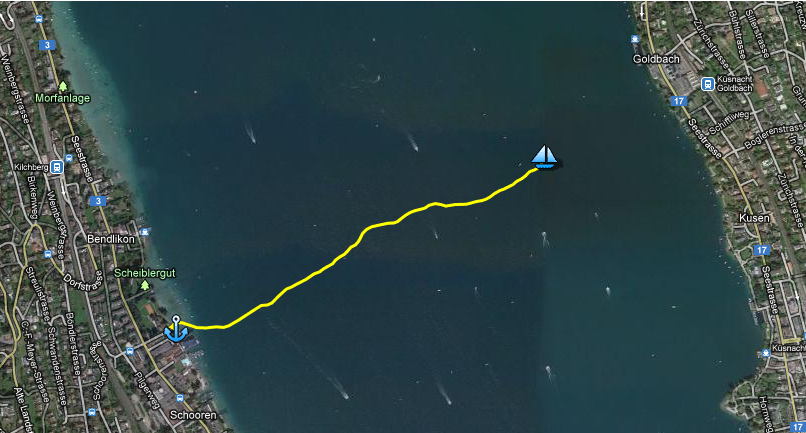
\includegraphics[width=4in]{figures/lake.png}}{www.limnobotics.ch}
}
\end{center}
\end{frame}

\begin{frame}
\begin{center}
\vspace{0.2in}
\includegraphics<1>[width=4.7in]{figures/limno_bgape_sc}
\includegraphics<2>[width=4.7in]{figures/limno_bgape}
\includegraphics<3>[width=4.7in]{figures/limno_bgape_ls}
\only<4>{\hspace{-2em}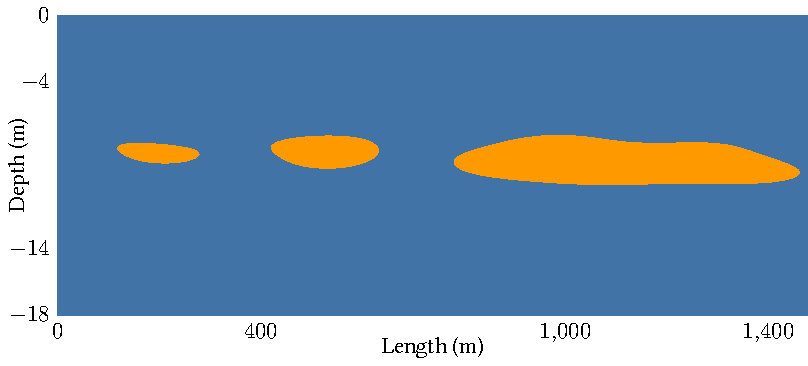
\includegraphics[width=4.45in]{figures/limno_bgape_cl}}
\end{center}
\end{frame}

\begin{frame}
\begin{itemize}
\item<1-> Pose as a sequential decision making problem (\emph{pool-based active learning}):
\begin{itemize}
\item<2-> No measurements available in advance, just a set (pool) of possible sampling locations ($D$)
\vspace{0.5em}
\item<3->[]\hspace{-1.5em} At each iteration $t \geq 1$:
\item<3-> Decide where to measure next ($x_t$)
\item<4-> Obtain noisy observation ($y_t = f(x_t) + n_t$)
\item<5-> Update our estimate of the underlying function (e.g. algae concentration)
\end{itemize}
\end{itemize}
\begin{center}
\color{white}
\includegraphics<1>[draft,width=4.45in]{figures/oned_0}
\color{black}
\includegraphics<2>[width=4.45in]{figures/oned_0}
\includegraphics<3>[width=4.45in]{figures/oned_1_0}
\includegraphics<4>[width=4.45in]{figures/oned_1_1}
\includegraphics<5>[width=4.45in]{figures/oned_1_2}
\includegraphics<6>[width=4.45in]{figures/oned_2_0}
\includegraphics<7>[width=4.45in]{figures/oned_2_1}
\includegraphics<8>[width=4.45in]{figures/oned_2_2}
\end{center}
\end{frame}

\begin{frame}
\begin{enumerate}
\item<1-> How do we \textbf{estimate} the function?
\vspace{1em}
\item<2-> How do we \textbf{classify}?
\vspace{1em}
\item<3-> Each measurement is expensive (time, battery power).\\
      How do we \textbf{select} ``informative'' measurements?
\end{enumerate}
\vspace{2em}
\begin{center}
\uncover<4->{\large
Gaussian processes to the rescue!
}
\end{center}
\end{frame}

\begin{frame}
\begin{center}
\uncover<1->{\large Why GPs are nice}
\end{center}
\begin{itemize}
\item<2-> \textbf{Nonparametric}:\\
      Impose ``smoothness'' assumptions via kernel $k(x, x')$.
\vspace{1em}
\item<3-> \textbf{Bayesian}, yet \textbf{efficient}:
      \begin{align*}
        \mu_t(\*x) &= \*k_t(\*x)^T\left(\*K_t + \sigma^2 \*I\right)^{-1}\*y_t\\
        k_t(\*x, \*x') &= k(\*x, \*x') - \*k_t(\*x)^T\left(\*K_t + \sigma^2 \*I\right)^{-1}\*k_t(\*x)\notag\\
        \sigma_t^2(\*x) &= k_t(\*x, \*x)
      \end{align*}
      Suitable for step-by-step updates.
\vspace{1em}
\item<4-> They provide \textbf{variance estimates}!\\
          Construct confidence intervals: $Q_t(\*x) = \left[\mu_{t-1}(\*x) \pm \beta_t^{1/2} \sigma_{t-1}(\*x)\right]$
\end{itemize}
\end{frame}

\begin{frame}
\begin{center}
\includegraphics<1>[width=4.45in]{figures/voned_0}
\includegraphics<2>[width=4.45in]{figures/voned_1_0}
\includegraphics<3>[width=4.45in]{figures/voned_1_1}
\includegraphics<4>[width=4.45in]{figures/voned_1_2}
\includegraphics<5>[width=4.45in]{figures/voned_2_0}
\includegraphics<6>[width=4.45in]{figures/voned_2_1}
\includegraphics<7>[width=4.45in]{figures/voned_2_2}
\includegraphics<8>[width=4.45in]{figures/voned_3_0}
\includegraphics<9>[width=4.45in]{figures/voned_3_1}
\includegraphics<10>[width=4.45in]{figures/voned_3_2}
\end{center}
\end{frame}

\begin{frame}
\begin{enumerate}
\item<1-> How do we \textbf{estimate} the function? \uncover<3->{\Large\color{green!70!black}\checkmark}
\vspace{0em}
\item<4-> How do we \textbf{classify}? \uncover<14->{\Large\color{green!70!black}\checkmark}
\vspace{0.3em}
\item<15-> How do we \textbf{select} ``informative'' measurements? \uncover<24->{\Large\color{green!70!black}\checkmark}
\uncover<16->{
\begin{itemize}
\item<16-> Pick among the yet unclassified.
\item<17-> Doesn't really matter which!\\
           \uncover<18->{(e.g. max. variance, }\uncover<19->{max. ambiguity}\uncover<23->{, or even random)}
\end{itemize}}
\end{enumerate}

\begin{center}
\color{white}
\includegraphics<1>[draft,width=3.5in]{figures/voned_cl_00}
\color{black}
\includegraphics<2-4>[width=3.5in]{figures/voned_cl_00}
\includegraphics<5>[width=3.5in]{figures/voned_cl_01}
\includegraphics<6>[width=3.5in]{figures/voned_cl_10}
\includegraphics<7>[width=3.5in]{figures/voned_cl_11}
\includegraphics<8>[width=3.5in]{figures/voned_cl_20}
\includegraphics<9>[width=3.5in]{figures/voned_cl_21}
\includegraphics<10>[width=3.5in]{figures/voned_cl_30}
\includegraphics<11>[width=3.5in]{figures/voned_cl_31}
\includegraphics<12>[width=3.5in]{figures/voned_cl_40}
\includegraphics<13-19>[width=3.5in]{figures/voned_cl_41}
\includegraphics<20>[width=3.5in]{figures/voned_cl_41_amb_0}
\includegraphics<21>[width=3.5in]{figures/voned_cl_41_amb_1}
\includegraphics<22->[width=3.5in]{figures/voned_cl_41_amb_2}
\end{center}
\end{frame}

\section{The LSE algorithm}
\definecolor{c1}{RGB}{255,255,255}
\definecolor{c2}{RGB}{27,161,226}
\definecolor{c6}{RGB}{140,191,38}
\definecolor{c4}{RGB}{240,150,9}
\definecolor{c5}{RGB}{255,255,255}
\definecolor{c3}{RGB}{230,113,184}
%\colorlet{c1}{cyan}
%\colorlet{c2}{magenta}
%\colorlet{c3}{red}
%\colorlet{c4}{green}
%\colorlet{c5}{yellow}

\begin{frame}
\begin{columns}[t]
\column{0.45\textwidth}
{\footnotesize
\begin{algorithmic}
  \REQUIRE sample set $D$, GP prior ($\mu_0$, $k$, $\sigma_0$),\\
           \hspace{2.2em}thr. value $h$, accuracy parameter $\epsilon$
  \ENSURE predicted sets $\hat{H}$, $\hat{L}$
  \uncover<2->{
  \CSTATE{c1}$H_0 \gets \varnothing$,\enskip $L_0 \gets \varnothing$,\enskip $U_0 \gets D$ \label{lin:init1}
  %\LET{$H_0$}{$\varnothing$} \label{lin:init1}
  %\LET{$L_0$}{$\varnothing$}
  %\LET{$U_0$}{$D$}
  \CLET{c1}{$C_0(\*x)$}{$\mathbb{R}$, for all $\*x \in D$} \label{lin:init2}
  \CLET{c1}{$t$}{1}
  }
  \uncover<3->{
  \CWHILE{c6}{$U_{t-1} \neq \varnothing$}
    \CSTATE{c6}$H_t \gets H_{t-1}$,\enskip $L_t \gets L_{t-1}$,\enskip $U_t \gets U_{t-1}$
    }
    %\LET{$H_t$}{$H_{t-1}$}
    %\LET{$L_t$}{$L_{t-1}$}
    %\LET{$U_t$}{$U_{t-1}$}
    \uncover<4->{
    \CFORALL{c2}{$\*x \in U_{t-1}$}
      \CLET{c2}{$C_{t}(\*x)$}{$C_{t-1}(\*x) \cap Q_t(\*x)$} \label{lin:upd}
      \CIF{c2}{$\min(C_t(\*x)) + \epsilon > h$} \label{lin:class1}
        \CLET{c2}{$U_t$}{$U_t \setminus \{\*x\}$}
        \CLET{c2}{$H_t$}{$H_t \cup \{\*x\}$} 
      \CELSIF{c2}{$\max(C_t(\*x)) - \epsilon \leq h$} \label{lin:classr2}
        \CLET{c2}{$U_t$}{$U_t \setminus \{\*x\}$}
        \CLET{c2}{$L_t$}{$L_t \cup \{\*x\}$}
      \CENDIF{c2} \label{lin:class2}
    \CENDFOR{c2}
    }
    \uncover<5->{
    \CLET{c3}{$\*x_t$}{$\argmax \{a_t(\*x)\mid \*x \in U_t\}$} \label{lin:sel1}
    \CLET{c3}{$y_t$}{$f(\*x_t) + n_t$} \label{lin:sel2}
    }
    \uncover<6->{
    \CSTATE{c4}Compute $\mu_t(\*x)$ and $\sigma_t(\*x)$, $\forall\*x \in U_t$ \label{lin:inf}
    }
    \uncover<3->{
    \CLET{c6}{$t$}{$t + 1$}
  \CENDWHILE{c6}
  }
  \uncover<2->{
  \CLET{c5}{$\hat{H}$}{$H_{t-1}$} \label{lin:ret1}
  \CLET{c5}{$\hat{L}$}{$L_{t-1}$} \label{lin:ret2}
  }
\end{algorithmic}
}
\column{0.55\textwidth}
\begin{center}
The Level Set Estimation (\acl) algorithm
\end{center}
\only<3-6>{\vspace{34pt}$\leftarrow$ {\small loop until all points have been classified\\}\vspace{40pt}}
\only<4-6>{$\leftarrow$ {\small classify\\}\vspace{52pt}}
\only<5-6>{$\leftarrow$ {\small select max. ambiguity point\\}\vspace{3pt}}
\only<6>{$\leftarrow$ {\small update GP estimate}}
\only<7->{
\vspace{3pt}
\begin{itemize}
\only<7->{
\item Monotonicity of
\begin{enumerate}
\item confidence intervals
\item classification
\end{enumerate}
}
\vspace{0em}
\only<8->{
\item Relaxed classification rules by an accuracy parameter $\epsilon$\\
      (trades off sampling cost for accuracy)
}
\end{itemize}
}
\begin{center}
\includegraphics<8->[width=2in]{figures/voned_cl_41_eps}
\end{center}
\end{columns}
\end{frame}

\begin{frame}
\begin{center}
\includegraphics<1->[width=4in]{figures/limno_bgape_ls}\\

\only<1>{\color{white}\small{$t = 0$\\}}
\only<2>{\small{$t = 0$\\}}
\only<3>{\small{$t = 20$\\}}
\only<4>{\small{$t = 40$\\}}
\only<5>{\small{$t = 60$\\}}
\only<6>{\small{$t = 80$\\}}
\only<7>{\small{$t = 100$\\}}
\only<8>{\small{$t = 120$\\}}
\only<9>{\small{$t = 140$\\}}
\only<10>{\small{$t = 160$\\}}
\only<11>{\small{$t = 180$\\}}
\only<12>{\small{$t = 200$\\}}
%\only<13>{\small{$t = 220$\\}}
%\only<14>{\small{$t = 240$\\}}
\only<13>{\small{$t = 260$\\}}
%\only<16>{\small{$t = 280$\\}}
%\only<17>{\small{$t = 300$\\}}
%\only<18>{\small{$t = 320$\\}}
%\only<19>{\small{$t = 340$\\}}
\only<14>{\small{$t = 354$\\}}



\hspace{-1.9em}
\color{white}
\includegraphics<1>[draft,width=3.78in]{figures/limno_bgape_class_20}
\color{black}
\includegraphics<2>[width=3.78in]{figures/limno_bgape_class_0}
\includegraphics<3>[width=3.78in]{figures/limno_bgape_class_20}
\includegraphics<4>[width=3.78in]{figures/limno_bgape_class_40}
\includegraphics<5>[width=3.78in]{figures/limno_bgape_class_60}
\includegraphics<6>[width=3.78in]{figures/limno_bgape_class_80}
\includegraphics<7>[width=3.78in]{figures/limno_bgape_class_100}
\includegraphics<8>[width=3.78in]{figures/limno_bgape_class_120}
\includegraphics<9>[width=3.78in]{figures/limno_bgape_class_140}
\includegraphics<10>[width=3.78in]{figures/limno_bgape_class_160}
\includegraphics<11>[width=3.78in]{figures/limno_bgape_class_180}
\includegraphics<12>[width=3.78in]{figures/limno_bgape_class_200}
%\includegraphics<13>[width=3.78in]{figures/limno_bgape_class_220}
%\includegraphics<14>[width=3.78in]{figures/limno_bgape_class_240}
\includegraphics<13>[width=3.78in]{figures/limno_bgape_class_260}
%\includegraphics<16>[width=3.78in]{figures/limno_bgape_class_280}
%\includegraphics<17>[width=3.78in]{figures/limno_bgape_class_300}
%\includegraphics<18>[width=3.78in]{figures/limno_bgape_class_320}
%\includegraphics<19>[width=3.78in]{figures/limno_bgape_class_340}
\includegraphics<14>[width=3.78in]{figures/limno_bgape_class_354}
\end{center}
\end{frame}

\subsection*{Theoretical analysis}
%\begin{frame}
%How do we judge the ``accuracy'' of a solution $(\hat{H}, \hat{L})$?
%\uncover<2->{
%\begin{definition}[Misclassification loss]
%%\begin{align*}
%$\ell_h(\*x) = \twopartdef{\max\{0, f(\*x) - h\}}{\*x\in \hat{L}}{\max\{0, h - f(\*x)\}}{\*x\in \hat{H}}$
%%\end{align*}
%\end{definition}
%\begin{center}
%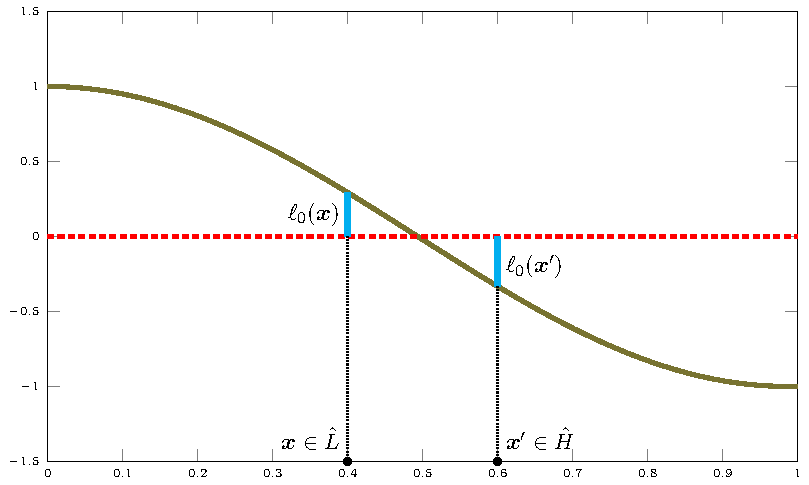
\includegraphics[width=3.5in]{figures/misclass}
%\end{center}
%}
%\end{frame}

%\begin{frame}
%\footnotesize
%\begin{tikzpicture}[node distance=1cm, auto,]
% \uncover<1->{
% \node[st] (conv) {Convergence};
% }
%
% \uncover<3->{
% \node[st,below=3em of conv] (clas) {All points in $D$ have been classified}
%   edge[pil] (conv);
% }
%
% \uncover<4->{
% \node[st,text width=14em,below=3em of clas] (amb)
% {\makecell[c]
%   {Conf. intervals ($\Leftrightarrow$ ambiguities)\\
%    get small enough ($<2\epsilon$)\uncover<12->{:\\[0.5em]
%    $a_t(\*x_t) \sim \mathcal{O}\left(\sqrt{\displaystyle\frac{\beta_t\gamma_t}{t}}\right)$
%    }
%   }
% } edge[pil] (clas);
% 
% \uncover<4->{ 
% \node[st,right=1.5em of clas] (eps) {$\epsilon$}
%   edge[pil] (amb);
% }
% 
% \uncover<18->{ 
% \node[st,right=1.5em of clas,fill=c6] (eps) {$\epsilon$}
%   edge[pil] (amb);
% }
% 
% \node[st,draw=none,below=3em of amb] (dummy) {};
% }
%
% \uncover<11->{
% \node[st,left=1.5em of amb] (t0) {Monotonicity}
%   edge[pil] (amb);
% }
% 
% \uncover<5->{
% \node[st,left=3em of dummy] (t1) {Samples ($t$)}
%   edge[pil] (amb);
% }
% 
% \uncover<6->{
% \node[st,right=1em of t1] (t2) {Kernel ($k$)}
%   edge[pil] (amb);
% }
% 
% \uncover<7->{
% \node[st,right=1em of t2] (t3) {Noise ($\sigma$)}
%   edge[pil] (amb);
% }
% 
% \uncover<8->{
% \node[st,right=3em of t3] (t4) {$\beta_t$}
%   edge[pil] (amb);
% }
% 
% \uncover<18->{
% \node[st,right=3em of t3,fill=c6] (t4) {$\beta_t$}
%   edge[pil] (amb);
% }
% 
% \uncover<9->{
% \node[draw=black,densely dotted,line width=0.7pt,fit=(t1)(t3)] (fit1) {};}
% 
% \uncover<9->{
% \node[st,below=3em of fit1] (gamma)
% {\makecell[c]
%   {Quantify by max. information gain (Srinivas \emph{et al.}, 2010):\\[0.5em]
%    $\gamma_t = \max_{\*y_t} I(\*y_{1:t}; f)$\uncover<10->{\\[0.5em]
%    For SE kernel $\gamma_t \sim \mathcal{O}\left((\log t)^{d+1}\right)$
%    }
%   }
% } edge[pil] (fit1);
% }
%
% \uncover<2->{
% \node[st,right=9em of conv] (acc) {Solution accuracy};
% }
%
% \uncover<14->{
% \node[st,below=3em of acc] (loss) {$\max_{\*x\in D} \ell_h(\*x) \leq \epsilon$}
%   edge[pil] (acc)
%   edge[pil,<-] (eps);
% }
%
% \uncover<15->{
% \node[st,right=1.5em of loss] (rules) {Class. rules}
%   edge[pil] (loss);
% }
%
% \uncover<16->{ 
% \node[st,below=3em of loss] (est) {Correctly estimate $f$ w.h.p.}
%   edge[pil] (loss);
% }
%
% \uncover<16->{ 
% \node[st,right=1.5em of est] (delta) {$\delta$}
%   edge[pil] (est);
% }
%
% \uncover<17->{
% \node[st,below=3em of est] (large) {Conf. intervals are large enough}
%   edge[pil] (est)
%   edge[pil,<-] (t4);
% }
%\end{tikzpicture}
%\end{frame}

%\begin{frame}
%\footnotesize
%\begin{tikzpicture}[node distance=1cm, auto,]
% \uncover<1->{
% \node[st] (conv) {Convergence};
% }
%
% \uncover<1->{
% \node[st,below=3em of conv] (clas) {All points in $D$ have been classified}
%   edge[pil] (conv);
% }
%
% \uncover<1->{
% \node[st,text width=14em,below=3em of clas] (amb)
% {\makecell[c]
%   {Conf. intervals ($\Leftrightarrow$ ambiguities)\\
%    get small enough ($<2\epsilon$)\uncover<1->{:\\[0.5em]
%    $a_t(\*x_t) \sim \mathcal{O}\left(\sqrt{\displaystyle\frac{\beta_t\gamma_t}{t}}\right)$
%    }
%   }
% } edge[pil] (clas);
% 
% \uncover<1->{ 
% \node[st,right=1.5em of clas] (eps) {$\epsilon$}
%   edge[pil] (amb);
% }
% 
% \uncover<1->{ 
% \node[st,right=1.5em of clas,fill=c6] (eps) {$\epsilon$}
%   edge[pil] (amb);
% }
% 
% \node[st,draw=none,below=3em of amb] (dummy) {};
% }
%
% \uncover<1->{
% \node[st,left=1.5em of amb] (t0) {Monotonicity}
%   edge[pil] (amb);
% }
% 
% \uncover<1->{
% \node[st,left=3em of dummy] (t1) {Samples ($t$)}
%   edge[pil] (amb);
% }
% 
% \uncover<1->{
% \node[st,right=1em of t1] (t2) {Kernel ($k$)}
%   edge[pil] (amb);
% }
% 
% \uncover<1->{
% \node[st,right=1em of t2] (t3) {Noise ($\sigma$)}
%   edge[pil] (amb);
% }
% 
% \uncover<1->{
% \node[st,right=3em of t3] (t4) {$\beta_t$}
%   edge[pil] (amb);
% }
% 
% \uncover<1->{
% \node[st,right=3em of t3,fill=c6] (t4) {$\beta_t$}
%   edge[pil] (amb);
% }
% 
% \uncover<1->{
% \node[draw=black,densely dotted,line width=0.7pt,fit=(t1)(t3)] (fit1) {};}
% 
% \uncover<1->{
% \node[st,below=3em of fit1] (gamma)
% {\makecell[c]
%   {Quantify by max. information gain (Srinivas \emph{et al.}, 2010):\\[0.5em]
%    $\gamma_t = \max_{\*y_t} I(\*y_{1:t}; f)$\uncover<1->{\\[0.5em]
%    For SE kernel $\gamma_t \sim \mathcal{O}\left((\log t)^{d+1}\right)$
%    }
%   }
% } edge[pil] (fit1);
% }
%
% \uncover<1->{
% \node[st,right=9em of conv] (acc) {Solution accuracy};
% }
%
% \uncover<1->{
% \node[st,below=3em of acc] (loss) {$\max_{\*x\in D} \ell_h(\*x) \leq \epsilon$}
%   edge[pil] (acc)
%   edge[pil,<-] (eps);
% }
%
% \uncover<1->{
% \node[st,right=1.5em of loss] (rules) {Class. rules}
%   edge[pil] (loss);
% }
%
% \uncover<1->{ 
% \node[st,below=3em of loss] (est) {Correctly estimate $f$ w.h.p.}
%   edge[pil] (loss);
% }
%
% \uncover<1->{ 
% \node[st,right=1.5em of est] (delta) {$\delta$}
%   edge[pil] (est);
% }
%
% \uncover<1->{
% \node[st,below=3em of est] (large) {Conf. intervals are large enough}
%   edge[pil] (est)
%   edge[pil,<-] (t4);
% }
%\end{tikzpicture}
%\end{frame}

\begin{frame}
\begin{theorem}[Convergence of \acl]
For any $h\in\mathbb{R}$, $\delta \in (0, 1)$, and $\epsilon > 0$,
if $\beta_t = 2\log(|D|\pi^2 t^2/(6\delta))$, \acl terminates after
at most $T$ iterations, where $T$ is the smallest positive integer
satisfying
\begin{align*}
\frac{T}{\beta_T \gamma_T} \geq \frac{C_1}{4\epsilon^2},
%T/(\beta_T \gamma_T) \geq C_1/(4\epsilon^2),
\end{align*}
where $C_1 = 8 / \log(1 + \sigma^{-2})$.

Furthermore, with probability at least $1-\delta$, the algorithm returns
an $\epsilon$-accurate solution, that is
\begin{align*}
\Pr\left\{\max_{\*x\in D}\ell_h(\*x) \leq \epsilon\right\} \geq 1 - \delta.
\end{align*}
\end{theorem}
\end{frame}

\begin{frame}
\begin{theorem}[Simplified]
If we choose $\beta_t$ large enough, then:
\begin{itemize}
\item<2-> \acl terminates after a number of iterations $T$
\begin{enumerate}
\item<3-> smoother kernel $\Rightarrow T \downarrow$
\item<4-> $\sigma \uparrow\ \Rightarrow T \uparrow$
\item<5-> ${\color<7>{red}\epsilon} \uparrow\ \Rightarrow T \downarrow$
\end{enumerate}
\item<6-> The solution returned is {\color<7>{red}$\epsilon$}-accurate with high probability
\end{itemize}
\end{theorem}
\end{frame}

\subsection*{Results}
\begin{frame}
\begin{center}
{\large Experiments}
\end{center}
\begin{enumerate}
\item \acl
\item<2-> Maximum variance sampling:
\vspace{-0.5em}
\begin{align*}
\*x_t = \argmax_{\*x\in D} \sigma_{t-1}(\*x)
\end{align*}
\item<3-> ``Straddle'' heuristic (Bryan \emph{et al.}, 2005):
\vspace{-0.5em}
\begin{align*}
\*x_t &= \argmax_{\*x\in D} 1.96\sigma_{t-1}(\*x)-|\mu_{t-1}(\*x) - h|\\
&\approx \argmax_{\*x\in D} a_{t-1}(\*x) \tag{for $\beta_t = 1.96$}
\end{align*}
\end{enumerate}
\end{frame}

\begin{frame}
\begin{center}
\hspace{4pt}\includegraphics<1->[width=4in]{figures/limno_chl_ls}\\[0.5em]
\uncover<2->{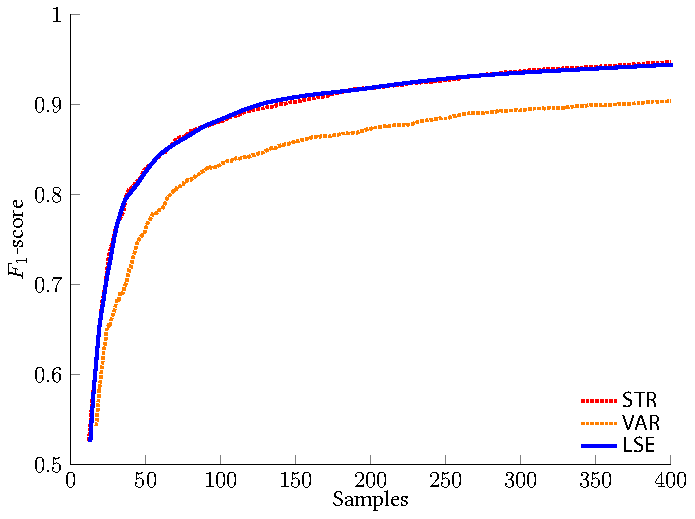
\includegraphics[width=2.3in]{figures/ev_chl_seq}}
\uncover<3>{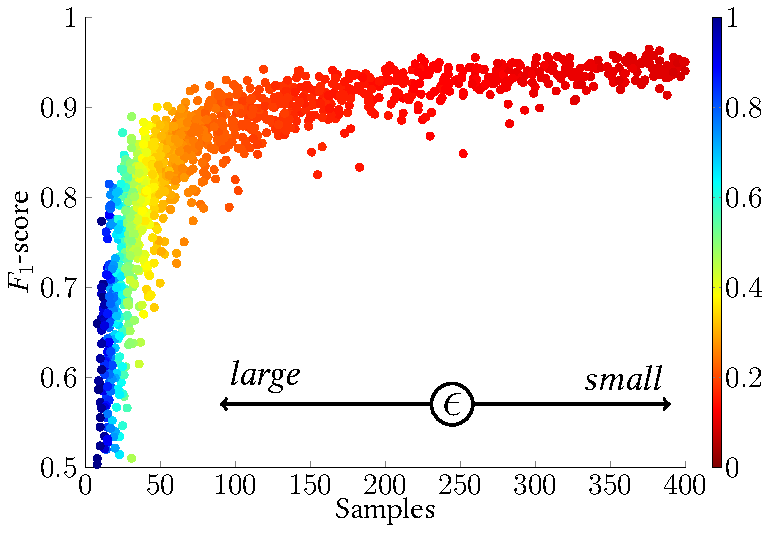
\includegraphics[width=2.3in]{figures/ev_chl_eps}}
\end{center}
\end{frame}

\begin{frame}
\begin{center}
\includegraphics<1->[width=4in]{figures/limno_bgape_ls}\\[0.5em]
\color{white}
\only<1>{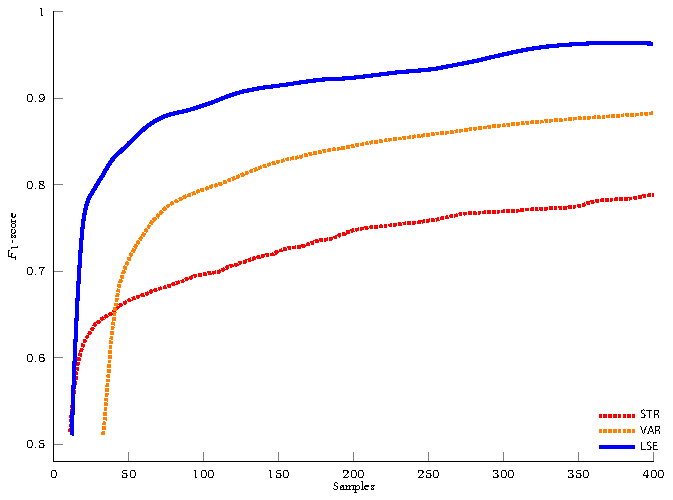
\includegraphics[draft,width=2.3in]{figures/ev_bgape_seq}}
\color{black}
\only<2-4>{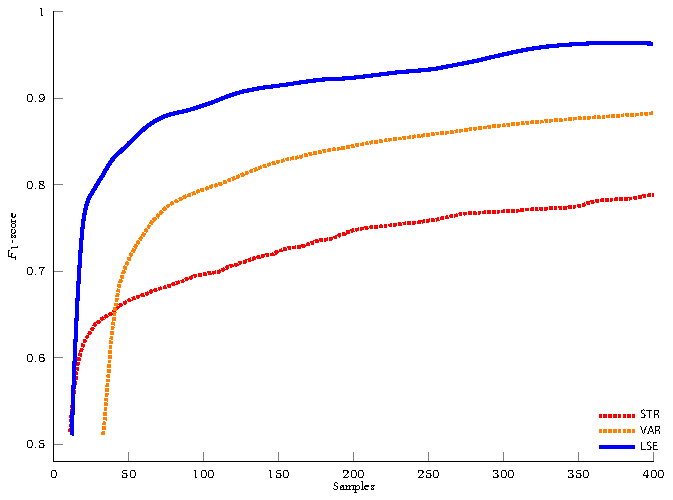
\includegraphics[width=2.3in]{figures/ev_bgape_seq}}
\color{white}
\only<2>{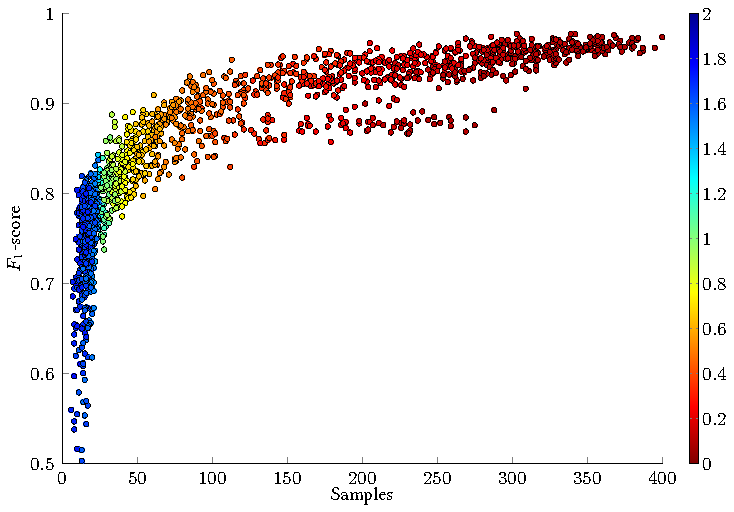
\includegraphics[draft,width=2.3in]{figures/ev_bgape_eps}}
\color{black}
\only<3>{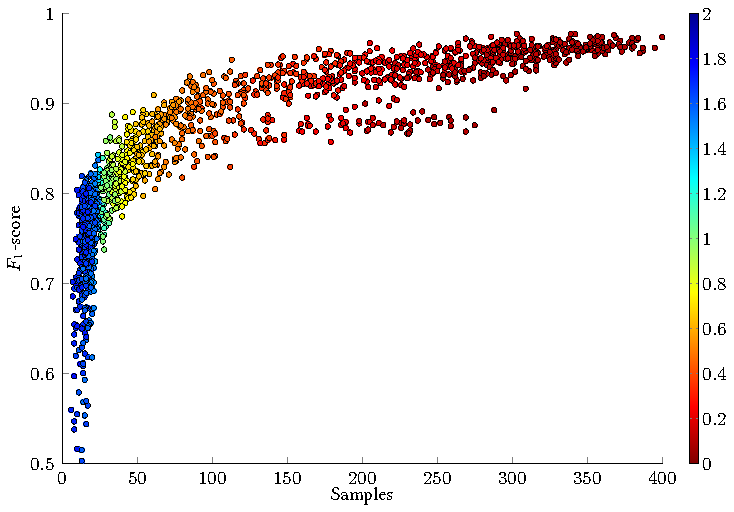
\includegraphics[width=2.3in]{figures/ev_bgape_eps}}
\only<4>{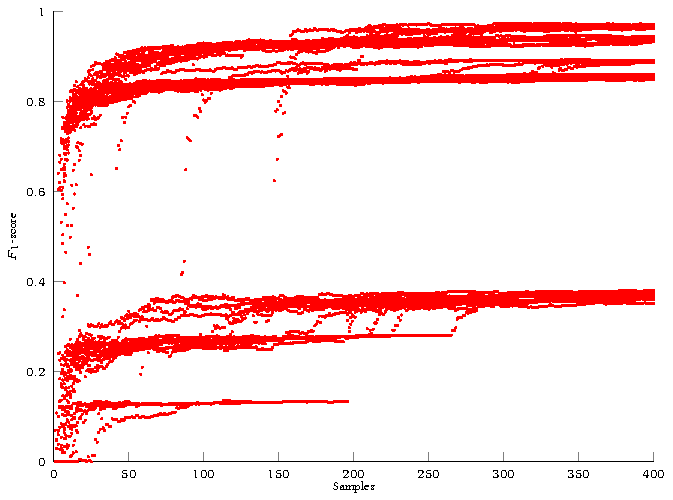
\includegraphics[width=2.3in]{figures/ev_bgape_seq_str_sc}}
\only<5>{\hspace{-16pt}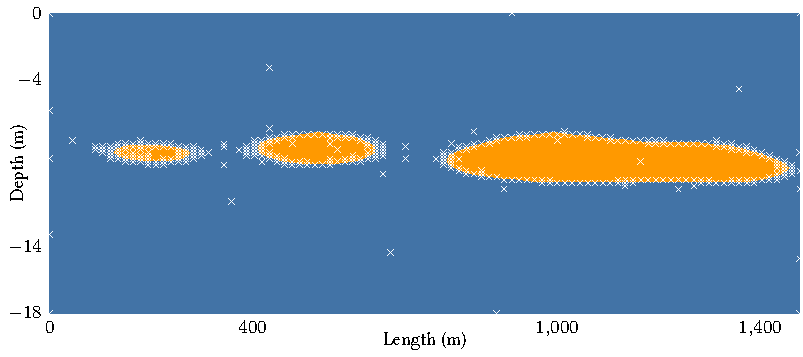
\includegraphics[width=3.77in]{figures/limno_bgape_class_354}}
\only<6>{\hspace{-16pt}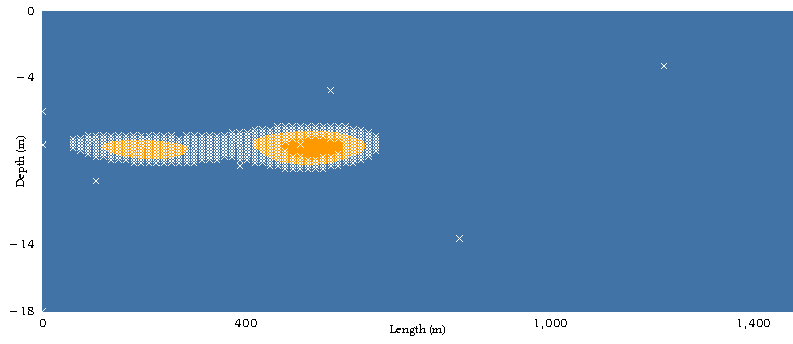
\includegraphics[width=3.77in]{figures/limno_bgape_str_class_400}}
\only<7>{\hspace{-16pt}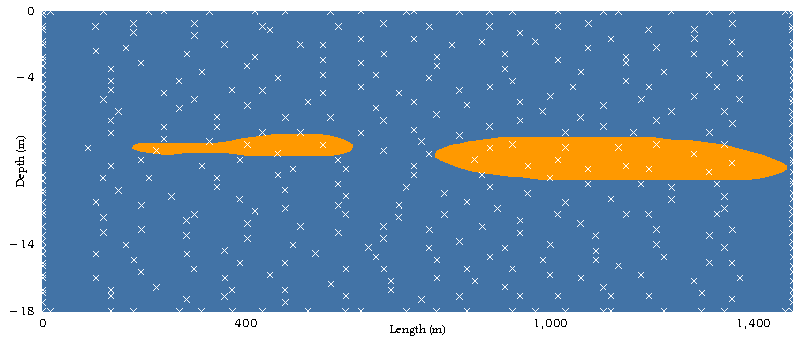
\includegraphics[width=3.77in]{figures/limno_bgape_var_class_400}}
\end{center}
\end{frame}

\section{Two extensions}

\begin{frame}
\begin{itemize}
\item<1-> What if we don't know $h$?
\item<2-> Implicitly define the threshold level: $h = \omega \max_{\*x\in D} f(\*x),\ 0 < \omega < 1$
\item<5-> \iacl:
\begin{itemize}
\item<5-> Need to accurately estimate the maximum (don't exclude points that could be maximizers)
\item<6-> Slower classification
\end{itemize}
\end{itemize}
\begin{center}
\color{white}
\only<1-2>{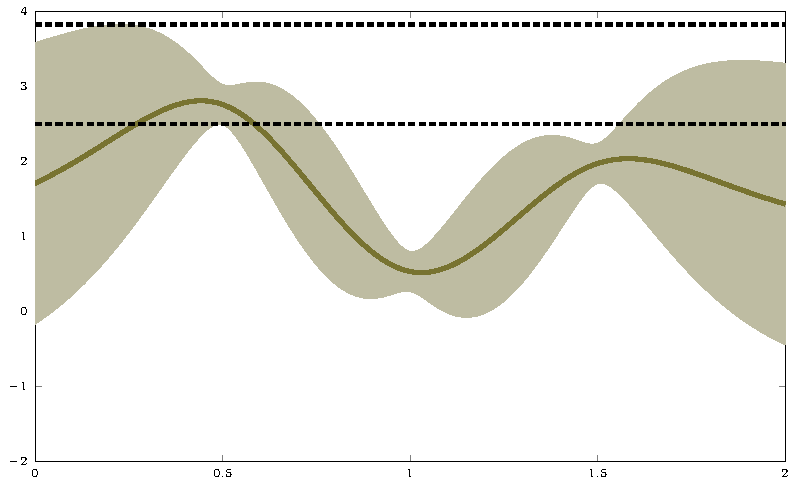
\includegraphics[draft,width=3.77in]{figures/voned_cl_41_imp_1}}
\color{black}
\only<3>{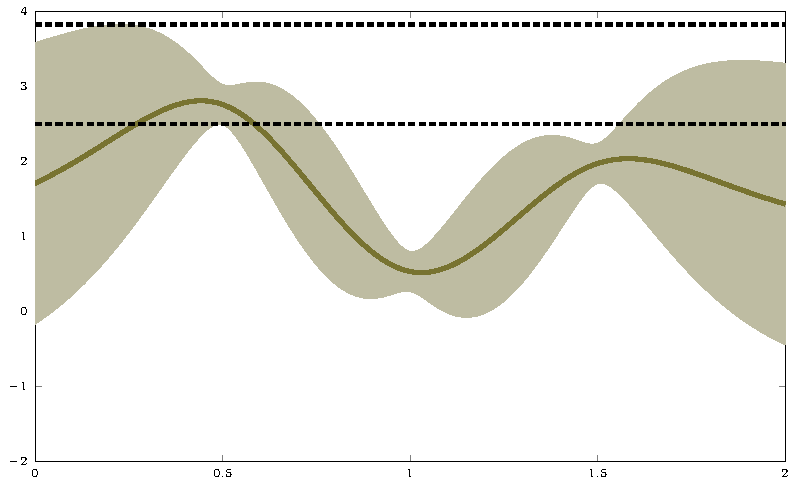
\includegraphics[width=3.77in]{figures/voned_cl_41_imp_1}}
\only<4->{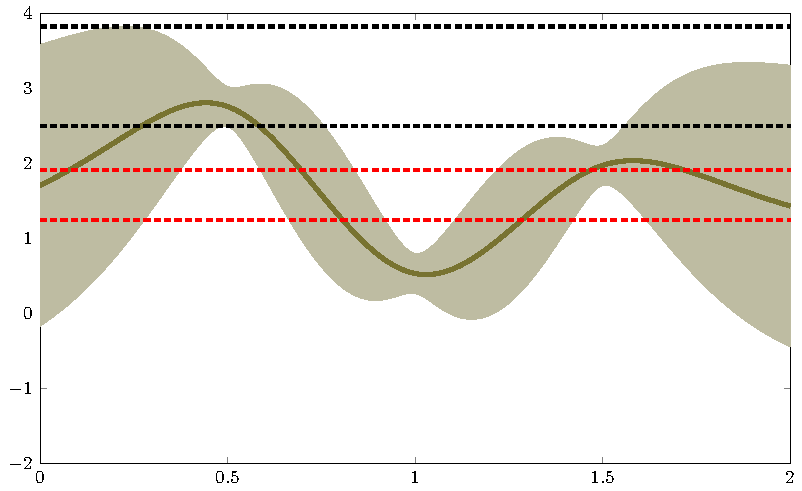
\includegraphics[width=3.77in]{figures/voned_cl_41_imp_2}}
\end{center}
\end{frame}

\begin{frame}
\begin{center}
\includegraphics<1-14>[width=4in]{figures/limno_bgape_ls}
\only<15>{\hspace{-1.9em}}
\includegraphics<15>[width=3.78in]{figures/limno_bgape_class_354}
\\

\only<1>{\color{white}\small{$t = 0$\\}}
\only<2>{\small{$t = 0$\\}}
\only<3>{\small{$t = 20$\\}}
\only<4>{\small{$t = 40$\\}}
\only<5>{\small{$t = 60$\\}}
\only<6>{\small{$t = 80$\\}}
\only<7>{\small{$t = 100$\\}}
\only<8>{\small{$t = 120$\\}}
\only<9>{\small{$t = 140$\\}}
\only<10>{\small{$t = 160$\\}}
\only<11>{\small{$t = 180$\\}}
\only<12>{\small{$t = 200$\\}}
%\only<13>{\small{$t = 220$\\}}
%\only<14>{\small{$t = 240$\\}}
\only<13>{\small{$t = 340$\\}}
%\only<16>{\small{$t = 280$\\}}
%\only<17>{\small{$t = 300$\\}}
%\only<18>{\small{$t = 320$\\}}
%\only<19>{\small{$t = 340$\\}}
\only<14>{\small{$t = 486$\\}}

\hspace{-1.9em}
\color{white}
\includegraphics<1>[draft,width=3.78in]{figures/limno_bgape_class_20}
\color{black}
\includegraphics<2>[width=3.78in]{figures/limno_bgape_imp_class_0}
\includegraphics<3>[width=3.78in]{figures/limno_bgape_imp_class_20}
\includegraphics<4>[width=3.78in]{figures/limno_bgape_imp_class_40}
\includegraphics<5>[width=3.78in]{figures/limno_bgape_imp_class_60}
\includegraphics<6>[width=3.78in]{figures/limno_bgape_imp_class_80}
\includegraphics<7>[width=3.78in]{figures/limno_bgape_imp_class_100}
\includegraphics<8>[width=3.78in]{figures/limno_bgape_imp_class_120}
\includegraphics<9>[width=3.78in]{figures/limno_bgape_imp_class_140}
\includegraphics<10>[width=3.78in]{figures/limno_bgape_imp_class_160}
\includegraphics<11>[width=3.78in]{figures/limno_bgape_imp_class_180}
\includegraphics<12>[width=3.78in]{figures/limno_bgape_imp_class_200}
\includegraphics<13>[width=3.78in]{figures/limno_bgape_imp_class_340}
\includegraphics<14->[width=3.78in]{figures/limno_bgape_imp_class_486}
\end{center}
\end{frame}

\begin{frame}
\begin{center}
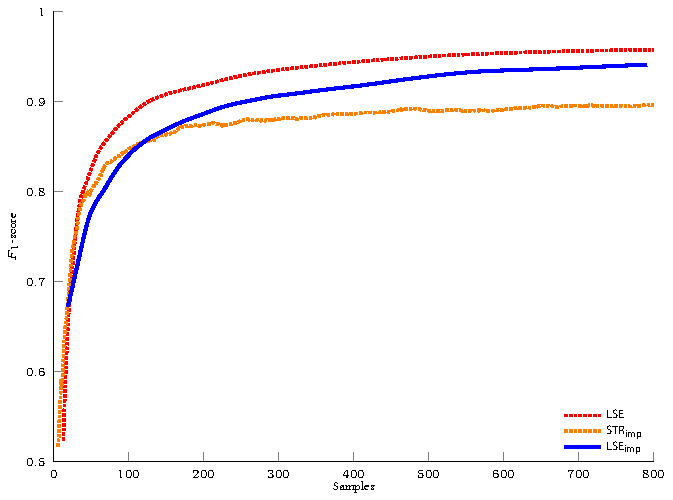
\includegraphics[width=2.3in]{figures/ev_chl_imp}
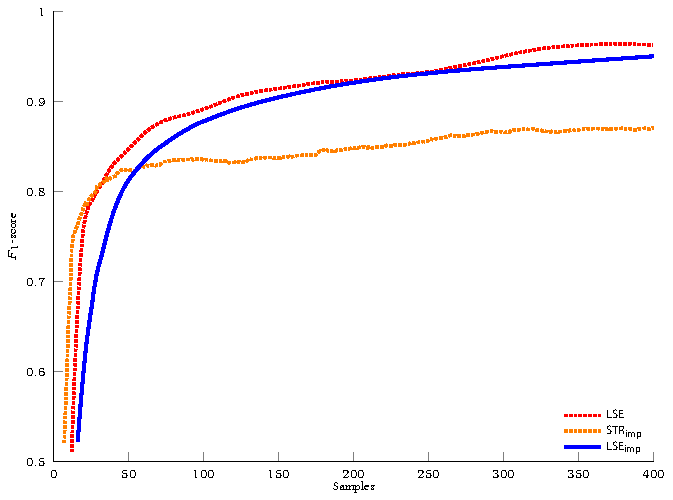
\includegraphics[width=2.3in]{figures/ev_bgape_imp}
\end{center}
\end{frame}

\begin{frame}
\begin{itemize}
\item<1-> Up to this point we have assumed a fixed cost per sample
\item<2-> What about the traveling distance between measurements?
\item<3-> Plan ahead:
\begin{itemize}
\item Select a \emph{batch} of sampling locations
\item Connect them using a Euclidean TSP path
\item Traverse path and collect measurements
\end{itemize}
\end{itemize}

\begin{center}
\color{white}
\includegraphics<1-3>[draft,width=3.78in]{figures/limno_bgape_pp_0_0}
\color{black}
\includegraphics<4>[height=1.8in]{figures/limno_bgape_pp_0_0}
\includegraphics<5>[height=1.8in]{figures/limno_bgape_pp_0_1}
\includegraphics<6>[height=1.8in]{figures/limno_bgape_pp_0_2}
\includegraphics<7>[height=1.8in]{figures/limno_bgape_pp_30_0}
\includegraphics<8>[height=1.8in]{figures/limno_bgape_pp_30_1}
\includegraphics<9>[height=1.8in]{figures/limno_bgape_pp_30_2}
\includegraphics<10>[height=1.8in]{figures/limno_bgape_pp_60_0}
\includegraphics<11>[height=1.8in]{figures/limno_bgape_pp_60_1}
\includegraphics<12>[height=1.8in]{figures/limno_bgape_pp_60_2}
\includegraphics<13>[height=1.8in]{figures/limno_bgape_pp_90_0}
\includegraphics<14>[height=1.8in]{figures/limno_bgape_pp_90_1}
\includegraphics<15>[height=1.8in]{figures/limno_bgape_pp_90_2}
\includegraphics<16>[height=1.8in]{figures/limno_bgape_pp_120_0}
\includegraphics<17>[height=1.8in]{figures/limno_bgape_pp_120_1}
\includegraphics<18>[height=1.8in]{figures/limno_bgape_pp_120_2}
\includegraphics<19>[height=1.8in]{figures/limno_bgape_pp_150_0}
\includegraphics<20>[height=1.8in]{figures/limno_bgape_pp_150_1}
\includegraphics<21>[height=1.8in]{figures/limno_bgape_pp_150_2}
\includegraphics<22>[height=1.8in]{figures/limno_bgape_pp_180_0}
\includegraphics<23>[height=1.8in]{figures/limno_bgape_pp_180_1}
\includegraphics<24>[height=1.8in]{figures/limno_bgape_pp_180_2}
\includegraphics<25>[height=1.8in]{figures/limno_bgape_pp_210_0}
\includegraphics<26>[height=1.8in]{figures/ev_bgape_pp}
\end{center}
\end{frame}

\section*{Conclusion}

\begin{frame}
\begin{center}
\large Summary
\end{center}
\vspace{-1em}
\begin{itemize}
\item<1-> \acl algorithm:
\begin{itemize}
\item<2-> \begin{tabular}{m{5.7cm} >{\centering}m{4cm}}Theoretical guarantees & 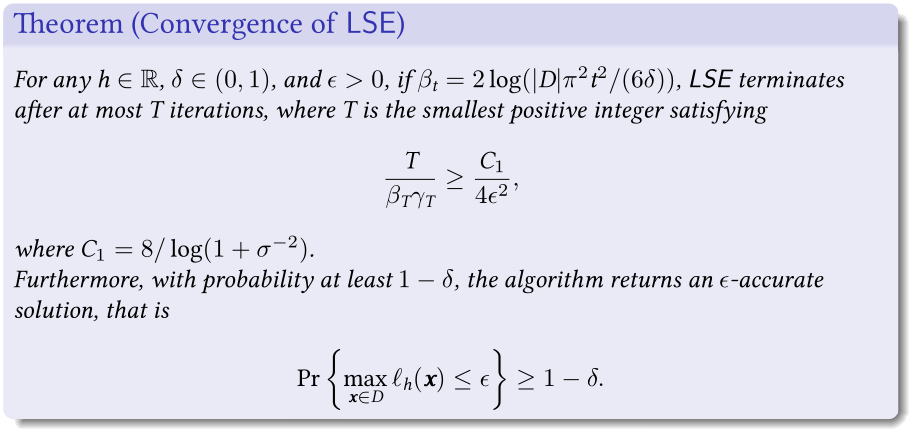
\includegraphics[width=1.3in]{figures/thm.png} \end{tabular}
\item<3-> \begin{tabular}{m{5.7cm} >{\centering}m{4cm}}Competitive with the state-of-the-art in practice (sometimes considerably superior) & \hspace{-0.5em}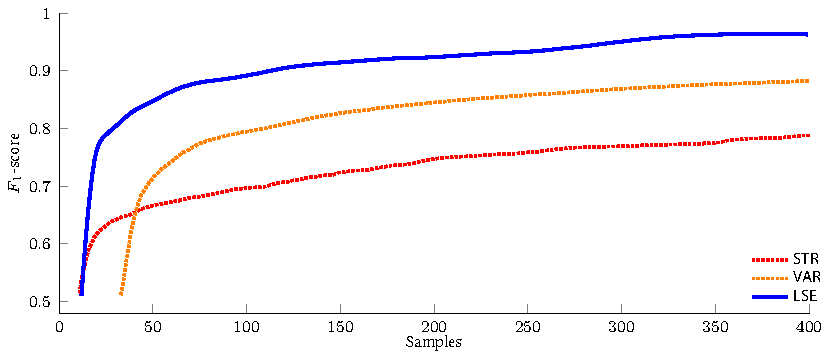
\includegraphics[width=1.3in]{figures/ev_bgape_seq_long} \end{tabular}
\end{itemize}
\item<4-> Two useful extensions:
\begin{itemize}
\item<5-> \begin{tabular}{m{5.7cm} >{\centering}m{4cm}}Implicit threshold level & 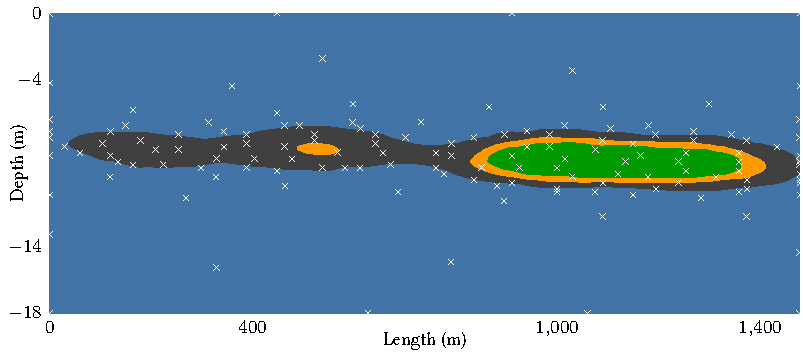
\includegraphics[width=1.3in]{figures/limno_bgape_imp_class_140} \end{tabular}
\item<6-> \begin{tabular}{m{5.7cm} >{\centering}m{4cm}}Batch sampling $\rightarrow$ path planning & 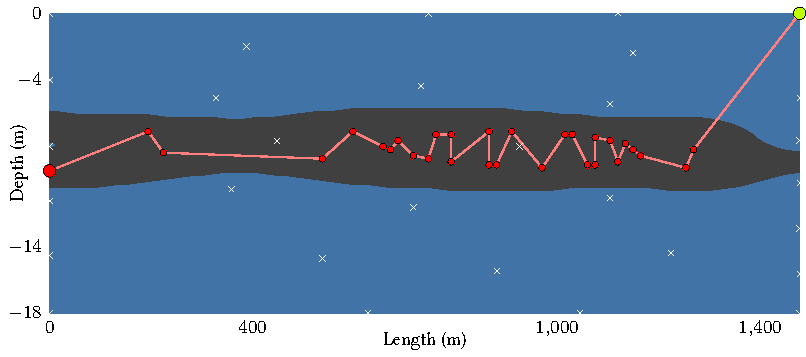
\includegraphics[width=1.3in]{figures/limno_bgape_pp_30_2} \end{tabular}
\end{itemize}
\item<7-> Look out for algae when swimming in Lake Zurich! =)
\end{itemize}
\end{frame}

\begin{frame}
\begin{center}
\large Questions?\\
\vspace{2em}
\sig{
\includegraphics[width=3in]{figures/dilbert}}{www.dilbert.com}
\end{center}
\end{frame}

\end{document}
